% !TeX program = xelatex
% !TeX encoding = utf-8
% 《机器人》LaTeX模板
% 面向往复夹持递送的血管介入机器人力反馈扰动建模与残差补偿

% 仅指定文档类路径，避免读入模板目录内其他稿件的编译缓存。
\documentclass{JQR_LaTeX_Template-0507/JQRnew}


% 修订标记：正文及公式按原稿逐段对照；干净版关闭颜色。
\providecommand{\RevisionColor}{\color{black}}
\newcommand{\revised}[1]{{\RevisionColor#1}}
\newcommand{\revbegin}{\begingroup\RevisionColor}
\newcommand{\revend}{\par\endgroup}

\JQRsetup{
 % 期刊出版信息
 volume     = xx,
 number     = x,
 year       = 2026,
 month      = 10,
 doi        = 240001,
 % 通信作者
 corrauthor = {\revised{胡琨元（Email：[待补]）；刘浩，Email: liuhao@sia.cn}},
 % 日期
 dates      = {2026-10-21/2026-10-21/2026-10-21},
 %
 % ---- 中文相关信息
 cntitle    = {面向往复夹持递送的血管介入机器人力反馈扰动建模与残差补偿},
 cnauthor   = {隋凯丞\addr{1,2,3}, 郑力铭\addr{1,2,3}, 林\quad 鹏\addr{1,2}, 胡琨元\addr{1,2*}, 刘\quad 浩\addr{1,2*}},
 runtitle   = {隋凯丞，等：面向往复夹持递送的血管介入机器人力反馈扰动建模与残差补偿},
 cnaddress  = {1. 中国科学院沈阳自动化研究所 机器人学国家重点实验室，辽宁~~沈阳\quad 110016；\\
               2. 辽宁省微创手术机器人重点实验室，辽宁~~沈阳\quad 110016；\\
               3. 中国科学院大学，北京\quad 100049},
 %
 % ----- 中文摘要
cnabstract = {\revbegin
夹持式血管介入机器人需要通过递送机构往复运动完成长距离递送，导致机构、器械力学状态改变，引起近端测力波动，影响术者对器械运动和受力状态的判断。针对这一问题，本文提出一种轴向力反馈重构方法，首先在在夹持切换期间保持切换前稳态载荷，递送机构恢复推进后，以传力链弹性加载与停顿后附加摩擦阻力衰减共同描述重新推进后的近端测力信号恢复过程。进一步，利用门控循环单元（GRU）编码单周期恢复过程，并通过跨周期注意力提取前序周期相同行程位置的编码特征，估计参考信号与物理模型补偿输出之间的残差。最后，通过程序及操作者进行模型实验，以验证方法有效性。实验结果表明，模型能够在间歇输送条件下提供稳定真实力觉感知，补偿后操作者任务表现上升。
\revend},
 % ---- 中文关键字
 cnkeywords = {\revised{介入机器人；往复夹持；轴向力反馈；载荷恢复；门控循环单元；跨周期注意力}},
 %
 % ---- 英文相关信息
 entitle    = {Disturbance Modeling and Residual Compensation of Force Feedback for Vascular Intervention Robot in Reciprocating Clamping Delivery},
 enauthor   = {\revised{SUI Kaicheng\addr{1,2,3}, ZHENG Liming\addr{1,2,3}, LIN Peng\addr{1,2}, HU Kunyuan\addr{1,2*}, LIU Hao\addr{1,2*}}},
 enaddress  = {1. \textit{State Key Laboratory of Robotics, Shenyang Institute of Automation, Chinese Academy of Sciences, Shenyang} 110016, \textit{China}; \\
               2. \textit{Key Laboratory of Minimally Invasive Surgical Robot, Liaoning Province, Shenyang} 110016, \textit{China}; \\
               3. \textit{University of Chinese Academy of Sciences, Beijing} 100049, \textit{China}},
 %
 % ---- 英文摘要
enabstract = {\revbegin
[Objective] To develop a force-feedback reconstruction method for proximal axial-force measurement fluctuations caused by alternating clamping in a vascular intervention robot. [Methods] During reciprocating delivery, the delivery and support mechanisms alternately clamp the instrument. After the support mechanism releases it, the delivery mechanism again carries the load alone and resumes forward delivery. The zero-load response term in the measured signal is corrected. Using forward travel as the independent variable, an axial load recovery model combines elastic loading of the force transmission chain with decay of additional frictional resistance after a hold. A gated recurrent unit (GRU) encodes each recovery process using the steady axial load before the mechanisms begin alternating clamping, the difference between this load and the initial load measured by the delivery mechanism after the support mechanism releases the instrument, mechanism motion, and forward travel. Cross-cycle attention aggregates features at corresponding travel positions in preceding cycles to estimate residuals not described by the physical model. Network inputs exclude real-time force measurements during recovery. [Results] Local peaks occurred in the recovery curves of most test cycles. When additional frictional resistance after a hold was included, the recovery model described local peaks and initial load changes. In offline resistance superposition tests, the proposed method fully preserved the added resistance during forward delivery after reloading. Feedback reconstruction errors and operator-task results are [待补]. [Conclusions] The method combines physical modeling and cross-cycle residual estimation to reconstruct axial force feedback during reciprocating clamping delivery.
\revend},
 %
 % ---- 英文关键字
 enkeywords = {\revised{intervention robot; reciprocating clamping; axial force feedback; load recovery; gated recurrent unit (GRU); cross-cycle attention}}
}

% ----- 加载宏包
\usepackage{algorithm}
\usepackage{algpseudocode}
\usepackage{pifont}
\usepackage{balance}
\usepackage{mwe}
\usepackage{booktabs}
\usepackage{amsmath,amssymb}
\usepackage{bm}
\usepackage{enumitem}
\usepackage{float}
\graphicspath{{JQR_LaTeX_Template-0507/}}
% 修订稿用 draft；干净稿改为 final。中文删除线支持自动换行。
\usepackage[draft,commentmarkup=footnote]{changes}
\usepackage{xeCJKfntef}
\setdeletedmarkup{\CJKsout{#1}}

\floatname{algorithm}{算法}
\renewcommand{\algorithmicrequire}{\textbf{输入:}}
\renewcommand{\algorithmicensure}{\textbf{输出:}}
\newcommand{\algorithmicchushi}{\textbf{初始化:}}

\begin{document}

\maketitle
% 栏底留白，避免通栏图下方正文被拉伸以强制对齐两栏底部。
\raggedbottom

% 引言部分不设节标题（遵循《机器人》期刊约定）
% 首栏由模板预留页脚空间，换栏时为第二栏预留相同高度。
\makeatletter
\AddToHookNext{cmd/@outputdblcol/after}{\JQRpubidadjcol}
\makeatother
血管介入机器人通过主从遥操作驱动导丝和导管完成推进与旋转，使术者能在导管室外远程完成介入手术操作，减少X射线辐射暴露\ucite{ref2}。但在遥操作中，术者无法通过指端感受器械阻力，而是需要通过力反馈功能来判断器械状态。接触力的测量影响着术者对器械受力状态的判断和操作，并进一步影响着手术的安全性\ucite{ref29}。力反馈既需要反映器械与环境之间的相互作用，也需要减少不必要的干扰波动，使术者能够辨别操作阻力的变化。

 从测量位置看，血管介入机器人相关的力感知可分为体内远端测力和体外近端测力。远端方案将体积较小的光纤布拉格光栅传感器\ucite{ref3,ref34}、压阻式传感器\ucite{ref35}集成于器械尖端，以获取局部接触载荷。这类方案需要兼顾器械尺寸、传感元件封装、弯曲性能与生物相容性，传感器集成也增加了器械制造与临床适配的复杂性。近端测力可通过驱动电机电流\ucite{ref5}估计器械载荷，也可在机构\ucite{ref4,ref12,ref36}中设置力传感器，此类布置保留了常规介入器械的末端结构，综合成本低、适配器械型号多。

滚轮式机构通过滚轮压紧器械，滚轮连续转动即可实现器械递送或撤出。Thakur等采用驱动轮与弹簧加载的从动滚轮配合推进导管\ucite{ref37}；Sankaran等通过滚轮驱动器械，并利用驱动电机电流估计近端操作力\ucite{ref5}；Chowdhury等利用双主动倾斜滚轮实现器械平移与旋转\ucite{ref38}。此类机构对器械的驱动力受到接触摩擦和压紧程度的限制，且易产生平移和旋转的运动耦合。

仿生手指夹持机构则通过相对设置的夹持面夹紧器械。Wang等设计了集成力感的多夹持器血管介入机器人\ucite{ref6}；Cao等设计了协同操作导丝和导管的多操作器\ucite{ref10}；Al-Ahmad等通过双编织套夹持器实现介入器械的连续运动\ucite{ref7}。以上机构均采用往复式递送，通过交替夹持，在有限的平移长度下实现器械长距离输送。由于使用近端测力方法时，器械载荷经递送机构的夹持组件和传力链传至测力元件，因此机构进行往复式递送时，测力元件受力状态随递送阶段改变，其中包含机构运动和承载状态变化的影响\ucite{ref9,ref12}。

针对机构运动和传力过程对力感知的影响，已有研究依据测力结构的受力关系建立补偿方法，通过测力部件的受力分析，建立与载荷、旋转速度相关的补偿关系\ucite{ref8}，或结合平移与旋转动力学、夹紧与松开状态下的对比测量及滤波，减小机构运行引起的测量误差\ucite{ref12}。学习方法也被用于机器人力感知，例如以机器人运动和软夹持器变形数据训练LSTM，估计柔性血管介入机器人的操作力和力矩\ucite{ref13}；Kim等采用GRU补偿六轴力/力矩传感器的温度漂移\ucite{ref39}；Zhou等将动力学模型与双阶段时序残差网络结合，补偿动力学模型和力估计误差\ucite{ref22}，这类方法能够捕捉到力学分析方法无法捕捉的未建模动态与高阶非线性信息，更好的实现估计或补偿。

由此，本文提出结合物理建模与残差学习的力反馈重构方法。分析承载切换引起的测量变化，区分测量值不反映外载的切换阶段与外载本身低于切换前稳态载荷的重新承载阶段，以弹性加载与停顿后附加摩擦阻力衰减描述重新推进时的轴向载荷恢复，并采用GRU及跨周期注意力估计物理模型未描述的残差。在机器人平台上开展程控递送实验与主从操作实验，评价重构误差、阻力响应及介入表现。文章第1节描述往复夹持递送过程与补偿目标，第2节介绍受力分析、轴向载荷恢复模型与反馈方法，第3节给出实验验证，第4节与第5节分别为讨论和结论。




\section{问题描述（Problem description）}

\subsection{往复夹持递送过程}


本文研究采用递送机构和支撑机构交替夹持器械的夹持式血管介入机器人。递送机构安装于沿直线导轨移动的滑台上，负责器械的轴向推进与周向旋转，并测量近端力；支撑机构安装于近血管鞘入口端，在递送机构释放与回退期间保持器械位置。

受直线导轨行程限制，这类机构长距离递送器械时，均采用周期性短行程往复运动完成。根据运动和夹持时序，将一个往复周期划分为S1～S10十个阶段，如图\ref{fig1}所示。
\begin{figure}[h]
\RevisionColor
\centering
\includegraphics[width=\linewidth]{图1.bmp}
\bicaption{\revised{往复夹持递送工作过程}}{\revised{Stages of reciprocating clamping delivery}}
\label{fig1}
\end{figure}
\begin{enumerate}[label=\arabic*),nosep,itemsep=0pt,topsep=2pt,partopsep=0pt,parsep=0pt,leftmargin=2\ccwd]
\item 递送与停止（S1～S2）：递送机构独立夹持器械推进，并可同时旋转（S1）；单次行程结束时滑台减速停止，支撑机构准备夹持器械（S2）。
\item 承载切换（S3～S4）：支撑机构夹持组件闭合，两个机构共同夹持器械（S3）；随后递送机构释放器械，由支撑机构承载（S4）。
\item 空载回程（S5～S6）：递送机构脱离器械后沿导轨退回（S5），在起点减速停止（S6），期间器械由支撑机构保持。
\item 重新承载与递送（S7～S10）：递送机构夹持器械，两机构再次共同夹持（S7）；支撑机构释放后，静止的递送机构独立承载（S8）；递送机构恢复前向推进，整体力学状态重新演化（S9）；力学状态恢复稳定，正常递送（S10）。
\end{enumerate}


\subsection{测力波动与补偿目标}

\revbegin
往复夹持递送使轴向测力通道周期性经历承载、卸载、重新承载并演化的过程。空载响应随旋转姿态变化；夹持组件开合冲击、停止后的载荷松弛及重新推进时的载荷恢复也会反映在近端测量信号中。
\revend

本文以近端力感获取的器械载荷作为补偿目标，重构往复夹持递送中的力反馈数值。通过力学分析及分阶段的处理策略，将往复运动中由于受力状态频繁改变而变动的力觉，补偿为相似运动条件、机构和器械条件、交互状态下的连续运动的力觉。

\revbegin
全文设轴向正方向沿器械名义中心轴指向远端，旋转角正方向遵循右手定则。力、扭矩、位移、角位移和时间的单位分别为 $\mathrm{N}$、$\mathrm{N}\cdot\mathrm{mm}$、$\mathrm{mm}$、$\mathrm{rad}$ 和 $\mathrm{s}$。轴向传感器读数记为 $F_{xm}$，扭矩传感器读数记为 $\tau_{xm}$。输出至主端的反馈信号统一记为 $\bm w_{\mathrm{fb}}=[F_{\mathrm{fb}},\tau_{\mathrm{fb}}]^{\rm T}$。
\revend



\section{受力分析与力反馈重构方法（Load transmission and feedback compensation for reciprocating clamping）}

\subsection{测量模型与承载切换中的载荷转移}

\revbegin
典型的递送机构的结构如图\ref{fig2}所示，通过某种传力组件，将器械与夹持组件的受力传递到力传感器中。对于这种机构，轴向力和绕轴扭矩满足
\revend
\begin{equation}
\label{eq:balance}
\begin{cases}
F_M+F_S=F_{\mathrm{out}},\\
\tau_M+\tau_S=\tau_{\mathrm{out}}.
\end{cases}
\end{equation}

\begin{figure}[h]
	\centering
	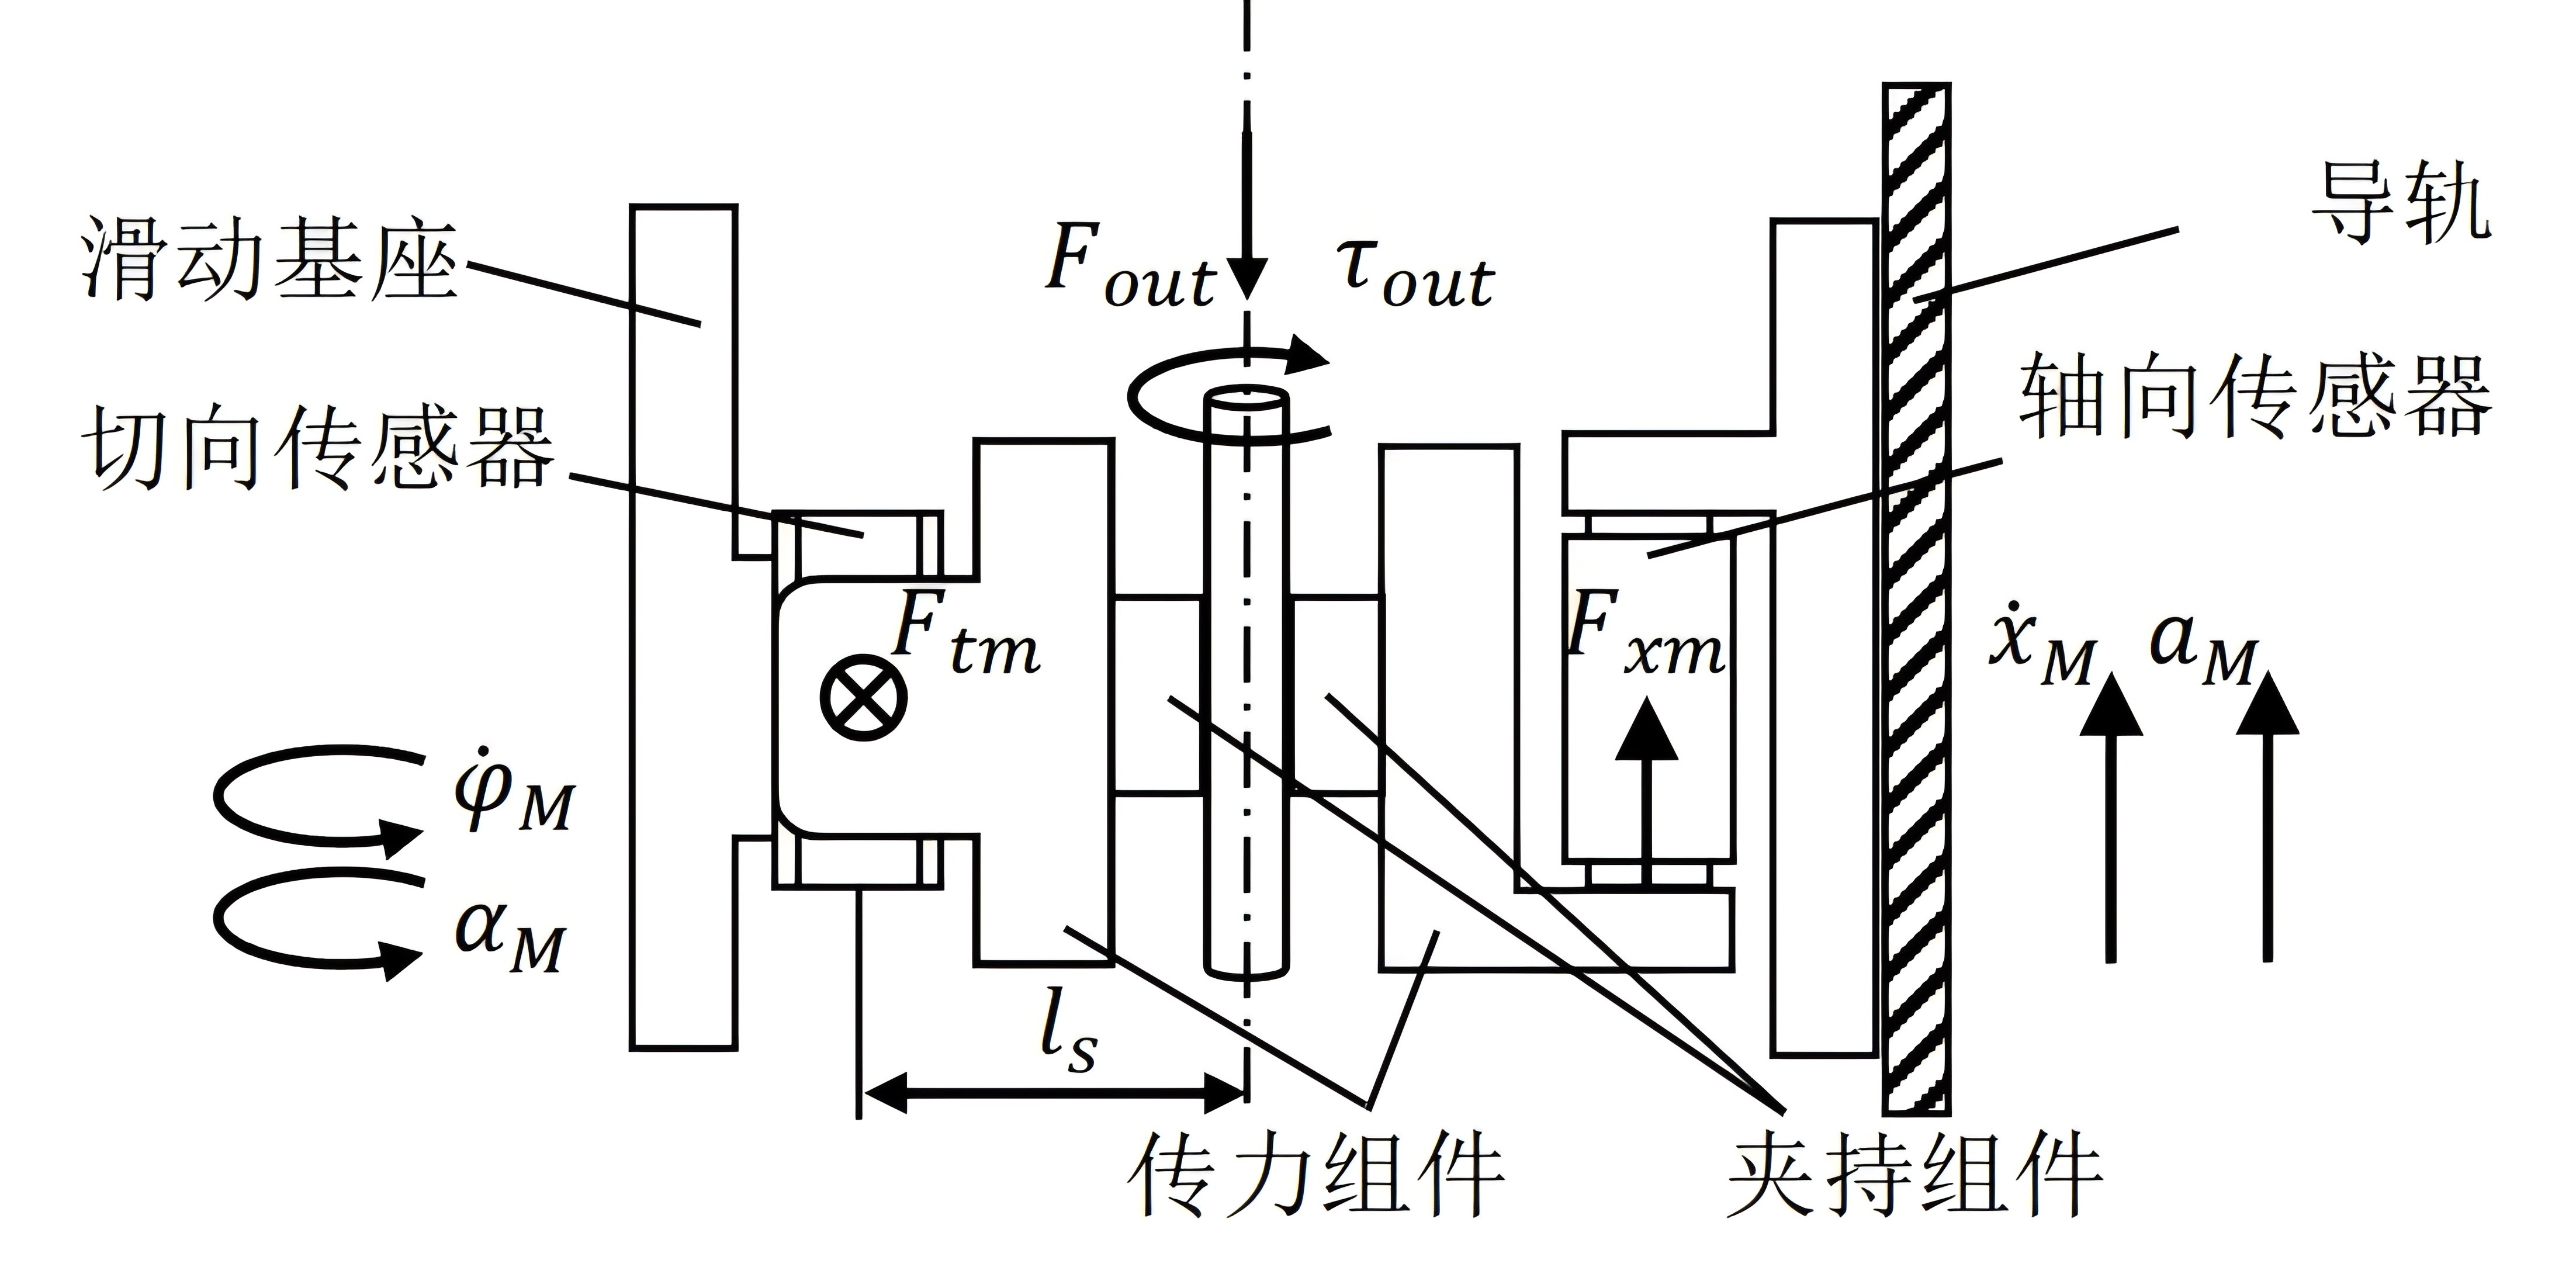
\includegraphics[width=\linewidth]{./figure2_manuscript.png}
	\bicaption{测力通道与递送机构、支撑机构的受力关系}{Force-sensing channels and load transfer between the delivery and support mechanisms}
	\label{fig2}
\end{figure}

式中，$F_M,\tau_M$ 与 $F_S,\tau_S$ 分别为递送机构和支撑机构作用于器械的轴向推力和驱动扭矩，$F_{\mathrm{out}},\tau_{\mathrm{out}}$ 为器械传导到近端的合阻力和合阻力矩，记 $\bm w_M=[F_M,\tau_M]^{\rm T}$。支撑机构完全释放时 $F_S=\tau_S=0$，外载全部由递送机构平衡。

\revbegin
将轴向力与换算后的扭矩组成测量向量 $\bm y=[F_{xm},\tau_{xm}]^{\rm T}$，传感器位于夹持、传力组件和滑台间，测量关系写为
\begin{equation}
\label{eq:measurement}
\bm y=\bm H_0\bm w_M+\bm b(\varphi_M)+\bm p(t)+\bm\varepsilon.
\end{equation}
式中，$\bm H_0\in\mathbb R^{2\times2}$ 为离线标定的可逆传递矩阵，反映了传感器读数与外部真实受力间的关系，以及轴向力和扭矩间的串扰，$\bm b(\varphi_M)$ 为空载响应项，包含静态零偏和随递送机构旋转角 $\varphi_M$ 变化的重力干扰，$\bm\varepsilon$ 为测量噪声，$\bm p(t)$ 为夹持组件开合引起的短时冲击。扣除空载响应项后的校正测量值为
\begin{equation}
\label{eq:corrected-measurement}
\tilde{\bm w}[k]=\bm H_0^{-1}\!\left[
\bm y[k]-\bm b(\varphi_M[k])\right].
\end{equation}
式中，$k$ 为离散采样时刻，对应时间为 $t_k$；$\tilde{\bm w}=[\tilde F,\tilde\tau]^{\rm T}$，$\tilde F$、$\tilde\tau$ 分别为轴向力和扭矩的校正测量值。

单机构递送阶段（S1、S2、S9、S10）支撑机构完全释放（$F_S=0$），递送机构独自平衡外载。S3～S7中支撑机构参与或独自承载（$F_S\neq0$），递送机构的测力通道在S4～S6卸载，并在S7重新参与承载。S7外载仍主要由支撑机构承担，，此时递送机构的测量值不反映外载，S8支撑机构释放后，静止的递送机构重新独自承载，此时器械静止，外载为器械与鞘管、血管壁之间静摩擦所平衡的残余载荷，由夹持组件、浮动传力组件及器械段组成的串联传力链中保留的变形决定。S2停止后的载荷松弛，以及S8递送机构承载时器械被夹持处向近端的微小移动，均使这部分变形减小，S8末递送机构实测载荷因而低于切换前的稳态值。

S1与S10输出校正测量值。S2滑台减速停止后载荷松弛，S3～S8的测量值又受承载切换和夹持组件开合冲击影响，均不代表连续递送时的器械载荷，这些阶段的反馈保持S1匀速段末的切换前稳态载荷向量
\begin{equation}
	\label{eq:lock}
	\bar{\bm w}=\frac{1}{N}
\sum_{j=k_1-N+1}^{k_1}
\tilde{\bm w}[j].
\end{equation}
式中，$k_1$ 为减速指令发出前的最后一个采样时刻，$N$ 为完全位于匀速段内的窗口长度，$\bar{\bm w}=[\bar F,\bar\tau]^{\rm T}$。取S8末支撑机构释放冲击衰减后、平移轴与旋转轴均静止（$\dot x_M=\dot\varphi_M=0$，$x_M$ 为递送机构的轴向位置）的采样时刻 $k_9$，以 $F_0=\tilde F[k_9]$ 作为S9起始时递送机构的轴向载荷，切换前后的轴向载荷差定义为待恢复载荷差：
\begin{equation}
	\label{eq:deficit}
	A=\bar F-F_0.
\end{equation}


\subsection{重新承载后的轴向载荷恢复模型}

恢复模型描述S9中整体力学状态重新演化的前向推进过程，即S8末减小的传力链变形尚未重新建立、器械与鞘管和血管壁之间尚未过渡至滑动摩擦的阶段。自S8末 $t_{k_9}$ 时刻起累计前向推进行程
\begin{equation}
\label{eq:recovery-travel}
s_{\mathrm r}(t)=\int_{t_{k_9}}^{t}
\max\!\left(\dot x_M(t'),0\right)\,\mathrm dt'.
\end{equation}
\revbegin

S9中的轴向载荷恢复包含两部分作用，一是递送机构重新承载后，夹持组件、浮动传力组件及器械段组成的串联传力链随推进逐步加载；二是器械在S2～S8静止后，与鞘管和血管壁之间形成的静摩擦需要转化为滑动摩擦，重新推进时形成附加阻力，并在一定滑移距离内过渡至滑动摩擦水平\ucite{dahl1968,ruina1983}，恢复过程及补偿量如图\ref{fig3}所示。以推进行程为自变量，令 $\hat F(s_{\mathrm r})$ 为模型给出的轴向载荷，采用一阶恢复关系
\revend
\begin{equation}
\label{eq:recovery-ode}
\frac{\mathrm d\hat F}{\mathrm ds_{\mathrm r}}
=\frac{\bar F+F_{\mathrm a}\mathrm e^{-s_{\mathrm r}/D_c}-\hat F}{\lambda}.
\end{equation}
\revbegin
式中，$\lambda>0$ 为弹性加载的特征行程，$F_{\mathrm a}\ge0$ 为停顿后附加摩擦阻力的幅值，$D_c>0$ 为附加阻力衰减的特征滑移距离。三个参数由辨识集的恢复曲线离线联合确定，在各周期的在线补偿中保持不变。以 $\hat F(0)=F_0$ 为初值积分，得到相对于切换前载荷的恢复补偿量
\revend
\begin{equation}
\label{eq:recovery-comp}
\begin{aligned}
f(s_{\mathrm r})&=\bar F-\hat F(s_{\mathrm r})\\
&=A\mathrm e^{-s_{\mathrm r}/\lambda}\\
&\quad-\frac{F_{\mathrm a}D_c}{D_c-\lambda}
\left(\mathrm e^{-s_{\mathrm r}/D_c}-\mathrm e^{-s_{\mathrm r}/\lambda}\right).
\end{aligned}
\end{equation}
当 $D_c=\lambda$ 时，取极限形式
\begin{equation}
\label{eq:equal-scales}
f(s_{\mathrm r})=
\left(A-F_{\mathrm a}\frac{s_{\mathrm r}}{\lambda}\right)\mathrm e^{-s_{\mathrm r}/\lambda}.
\end{equation}
\revbegin
当 $F_{\mathrm a}=0$ 时，只剩弹性加载项，载荷单调趋近切换前载荷。若不计弹性加载项（$\lambda\to0$），载荷在重新推进起点即跳回切换前载荷附近，与S8末实测的待恢复载荷差不符。若恢复曲线出现高于切换前载荷的局部峰值，$f$ 在局部峰值附近为负，即从实测值中扣除附加阻力分量。
\revend

令式\eqref{eq:recovery-ode}右端为零，得到局部峰值对应的行程
\begin{equation}
\label{eq:peak-location}
\begin{aligned}
s^*&=\frac{\lambda D_c}{D_c-\lambda}
\ln\frac{(A+B)D_c}{B\lambda},\\
B&=\frac{F_{\mathrm a}D_c}{D_c-\lambda}.
\end{aligned}
\end{equation}
\revbegin
对于 $A>0$、$F_{\mathrm a}>0$，$D_c>\lambda$ 时存在位于有限行程内的局部峰值；$D_c<\lambda$ 时还需满足 $A<F_{\mathrm a}D_c/(\lambda-D_c)$。两尺度相等时，$s^*=\lambda(1+A/F_{\mathrm a})$；$F_{\mathrm a}=0$ 时载荷单调趋近参考值。
\revend

\begin{figure}[!t]
\centering
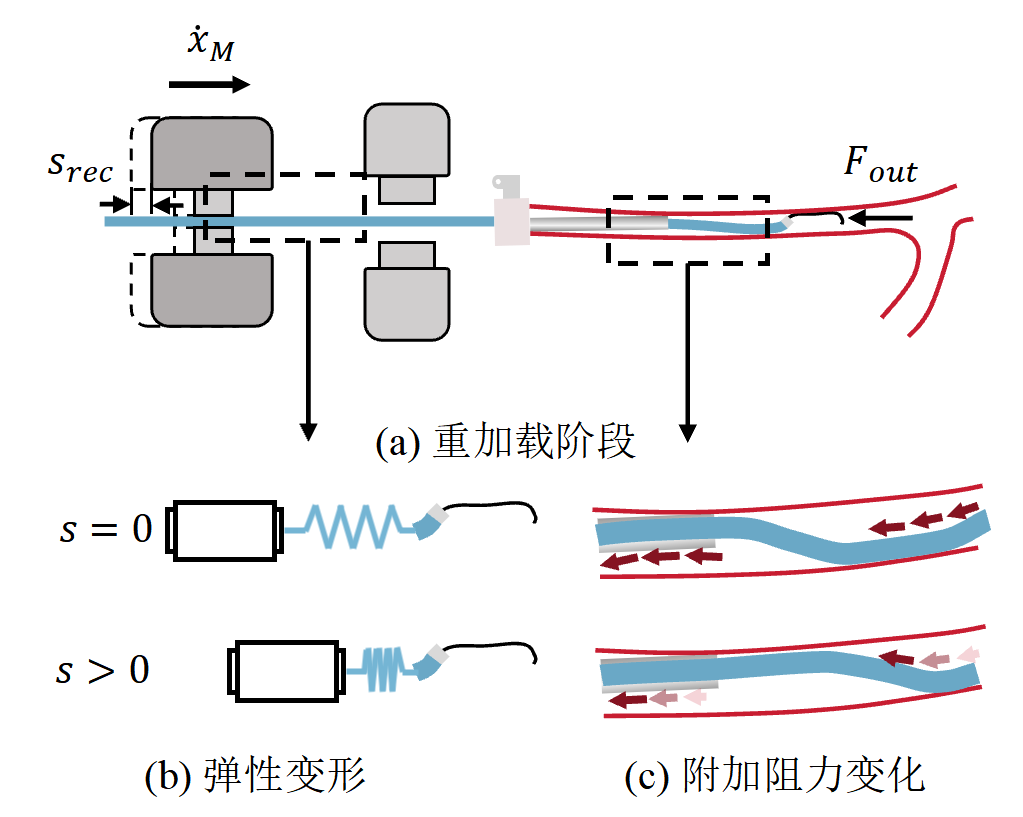
\includegraphics[width=\linewidth]{./figure3_manuscript.png}
\bicaption{轴向载荷恢复与补偿量示意}{Axial load recovery and the compensation term}
\label{fig3}
\end{figure}



\subsection{两级残差估计网络与分阶段反馈}

由于器械介入深度变化，会引起器械传力路径增长、摩擦状态变化，导致S9阶段加载状态变化，因此，引入残差估计网络，结合插入深度和前序周期信息修正模型补偿量。轴向物理模型输出由校正测量值与恢复补偿量组成：
\begin{equation}
\label{eq:physical-model-output}
F_{\mathrm p}[k]=\tilde F[k]
+\mathbb I_{\mathrm r}[k]f(s_{\mathrm r}[k]).
\end{equation}
式中，$\mathbb I_{\mathrm r}=1$ 表示S9中已启用且尚未开始撤除的恢复补偿，其余情况为0。补偿启用时，物理模型输出在恢复起点满足 $F_{\mathrm p}[k_9]=\bar F$。

残差估计网络用于估计恢复模型未描述的轴向残差。逐点输入为
\begin{equation}
\label{eq:gru-input}
\bm x_k=\big[\bar F,A,t_h,
\bm u_M[k]^{\rm T},s_{\mathrm r}[k],s[k],\sigma[k]\big]^{\rm T}..
\end{equation}
\revbegin
式中，$t_h$ 为S2滑台停止至S9开始的静止时长；$\bm u_M[k]$ 为递送机构平移与旋转的速度和加速度；$s[k]$ 为插入深度，用于描述随插入位置变化的残差；$\sigma[k]=\operatorname{sgn}\dot x_M[k]$ 为运动方向。$t_h$ 与 $\bar F$、$A$ 一样在本次S9开始时确定，网络不使用S9的实时测力值。。
\revend

前序周期恢复过程中的运动与承载切换时确定的载荷量可能影响本次恢复时的接触状态，因此采用两级网络引入这些历史信息。第一级在单个恢复过程内按推进行程的先后编码；第二级对前序周期同一行程位置的编码进行加权聚合。

记第 $c$ 个往复周期的S9为第 $c$ 个恢复过程，$c$ 为该周期在试次中的序号。将S9起点之后长度为 $s_{\mathrm w}$ 的前向行程等分为 $M$ 个行程单元，第 $m$ 个行程单元的样本集合为
\begin{equation}
\label{eq:phase}
\begin{aligned}
\Omega_{c,m}&=\big\{k\in\mathrm{S9}^{(c)}:(m-1)\Delta s\le s_{\mathrm r}[k]<m\Delta s\big\},\\
\Delta s&=s_{\mathrm w}/M,\quad m=1,\cdots,M.
\end{aligned}
\end{equation}
$s_{\mathrm w}$ 为统一的恢复补偿行程窗口，依据辨识数据选定，并在训练与测试中固定。该窗口用于确定参考配对区间、网络编码范围和正常推进时的补偿撤除位置。行程单元内无样本时，沿用前一行程单元的特征；首个行程单元无样本时取本周期起点输入。以起点输入初始化GRU，行程单元特征与编码为
\begin{equation}
\label{eq:cell-encoder}
\begin{aligned}
\bm h_{c,0}&=\mathrm{GRU}\big(\bm x_{k_9},\bm 0\big),\\
\bm z_{c,m}&=\frac{1}{|\Omega_{c,m}|}\sum_{k\in\Omega_{c,m}}\bm x_k,\\
\bm h_{c,m}&=\mathrm{GRU}\big(\bm z_{c,m},\bm h_{c,m-1}\big),
\end{aligned}
\end{equation}
式中，$\bm x_{k_9}$ 为本周期S9起点输入，初始化与后续行程单元编码共用同一组GRU参数\ucite{ref26}。$\bm h_{c,m}$ 在 $s_{\mathrm r}$ 到达行程单元终点 $m\Delta s$ 时计算。

% 通栏图4：由最终版 SVG 转为矢量 PDF，按原图175 mm宽度居中排在页顶。
\begin{figure*}[!t]
\centering
\makebox[\textwidth][c]{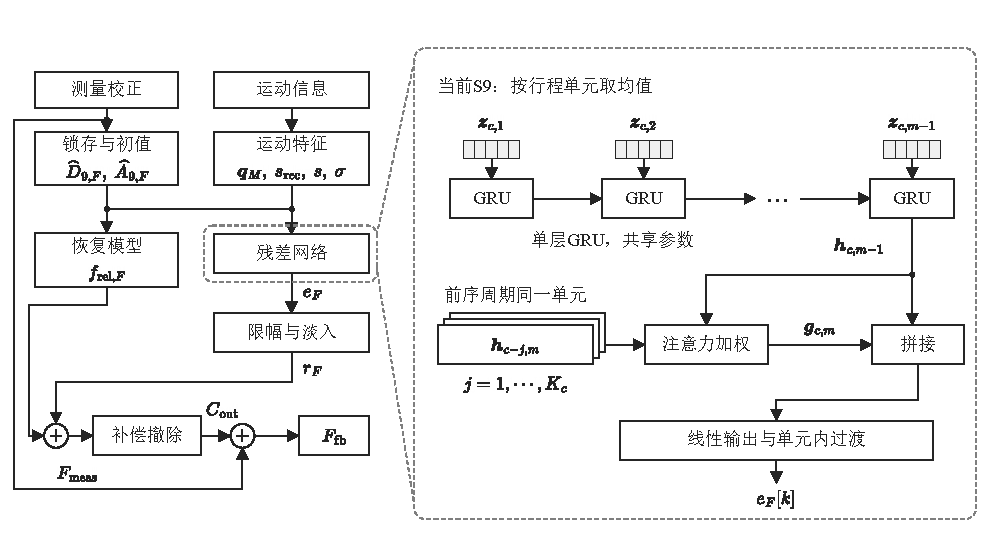
\includegraphics[width=175mm]{./Fig4_最终版.pdf}}
\bicaption{轴向力重构的反馈流程与两级残差估计网络}{Feedback scheme and two-level residual estimation network for axial force reconstruction}
\label{fig4}
\end{figure*}

第二级以当前周期上一行程单元结束时的编码为查询，以此前 $K_c$ 个周期第 $m$ 个行程单元的编码为键和值：
\begin{equation}
\label{eq:cross-cycle}
\begin{aligned}
\bm q_{c,m}&=\bm W_q\bm h_{c,m-1},\\
\bm\kappa_j&=\bm W_k\bm h_{c-j,m},\quad
\bm\upsilon_j=\bm W_v\bm h_{c-j,m},\\
\alpha_j&=\frac{\exp\!\left(\bm q_{c,m}^{\rm T}\bm\kappa_j/\sqrt d\right)}
{\sum_{j'=1}^{K_c}\exp\!\left(\bm q_{c,m}^{\rm T}\bm\kappa_{j'}/\sqrt d\right)},\\
\bm g_{c,m}&=\sum_{j=1}^{K_c}\alpha_j\bm\upsilon_j.
\end{aligned}
\end{equation}
式中，$\bm W_q$、$\bm W_k$、$\bm W_v$ 为查询、键和值的投影矩阵，$\alpha_j$ 为第 $c-j$ 个周期的注意力权重，$K_c=\min(K,c-1)$，$K$ 为历史周期数上限，$d$ 为编码维度，注意力为单头。$K_c=0$ 时取 $\bm g_{c,m}=\bm 0$，网络只使用当前周期的信息。前序周期第 $m$ 个行程单元的编码在该周期内已经算出，因此第 $m$ 个行程单元的残差估计在进入该行程单元时即可得到：
\begin{equation}
\label{eq:cell-output}
\hat e_{c,m}=\bm w_o^{\rm T}
\begin{bmatrix}\bm h_{c,m-1}\\\bm g_{c,m}\end{bmatrix}+b_o .
\end{equation}
式中，$\bm w_o$、$b_o$ 为输出层的权重和偏置。逐点残差在行程单元内由前一行程单元的估计线性过渡到本行程单元的估计：
\begin{equation}
\label{eq:cell-interp}
\begin{aligned}
e[k]&=(1-\mu_k)\,\hat e_{c,m-1}+\mu_k\,\hat e_{c,m},\quad k\in\Omega_{c,m},\\
\mu_k&=\frac{s_{\mathrm r}[k]-(m-1)\Delta s}{\Delta s},
\end{aligned}
\end{equation}
式中，$\hat e_{c,0}=0$。残差估计只依赖已经发生的运动，当前周期的运动信息相对输出滞后约一个行程单元长度。达到 $s_{\mathrm w}$ 后，按下述规则撤除补偿。

前序周期的编码由运动量和承载切换时确定的载荷量计算，不含S9的实时测力。训练和测试时，每个恢复过程都只使用同一试次中此前已经完成的周期。试次开头的周期没有历史（$K_c=0$），其误差单独统计。残差限幅与残差权重逐步增加规则为
\begin{equation}
\label{eq:residual-limit}
\begin{aligned}
e_{\max}&=\eta A+e_0,\\
r[k]&=\beta_k\operatorname{sat}(e[k],e_{\max}),\\
\beta_k&=\min\!\left\{1,\max\!\left[0,\frac{k-k_9}{N_b}\right]\right\}.
\end{aligned}
\end{equation}
式中，$e_{\max}$ 为残差限幅值，$r[k]$ 为残差修正量，$\beta_k$ 为残差权重，$\operatorname{sat}(e,a)=\max(-a,\min(e,a))$，$\eta\ge0$ 为限幅比例，$e_0>0$ 为最小限幅，$N_b$ 为残差权重逐步增加所需的采样点数。恢复补偿和残差修正仅在 $A>0$ 时启用。

正常恢复阶段的总补偿量为 $C[k]=f(s_{\mathrm r}[k])+r[k]$，轴向反馈为
\begin{equation}
\label{eq:active-output}
F_{\mathrm{fb}}[k]=\tilde F[k]+C[k].
\end{equation}
补偿启用时 $\beta_{k_9}=0$，故 $F_{\mathrm{fb}}[k_9]=\bar F$，与切换期间保持的输出衔接。实测值以单位权重进入输出，新增的外部阻力直接反映在反馈中。

当 $s_{\mathrm r}\ge s_{\mathrm w}$，或前向速度低于 $v_{\min}$ 持续超过 $T_{\mathrm{st}}$，或出现 $\dot x_M<-v_{\min}$ 的回拉时，开始撤除补偿。记触发时刻为 $t_e$，保存触发前最后一个有效补偿量 $C_e$，随后输出
\begin{equation}
\label{eq:withdrawal}
\begin{aligned}
F_{\mathrm{fb}}[k]&=\tilde F[k]+\rho_kC_e,\\
\rho_k&=\max\!\left\{0,1-\frac{t_k-t_e}{T_{\mathrm{off}}}\right\}.
\end{aligned}
\end{equation}
式中，$v_{\min}$ 为最小有效前向速度，$T_{\mathrm{st}}$ 为停止判定时长，$T_{\mathrm{off}}$ 为补偿撤除时长。撤除期间恢复模型与残差估计网络的输出不再更新；$\rho_k=0$ 后只输出校正测量值。因停止或回拉而退出时，本次恢复补偿不再重新启用。正常推进达到窗口终点并撤除补偿后进入S10。

令 $C_{\mathrm{out}}[k]$ 在正常恢复时为 $C[k]$，撤除时为 $\rho_kC_e$，未启用或已撤除时为0。全周期反馈为
\begin{equation}
\label{eq:phase-output}
\bm w_{\mathrm{fb}}[k]=
\begin{cases}
\bar{\bm w},&k\in\mathrm{S2}\sim\mathrm{S8},\\
\begin{bmatrix}\tilde F[k]+C_{\mathrm{out}}[k]\\
\tilde\tau[k]\end{bmatrix},&k\in\mathrm{S9},\\
\tilde{\bm w}[k],&k\in\{\mathrm{S1},\mathrm{S10}\}.
\end{cases}
\end{equation}
当 $A\le0$ 时，S9的 $C_{\mathrm{out}}=0$。扭矩在S9直接输出校正测量值。

网络监督采用的参考载荷取同一器械、鞘管和模型路径下，匹配插入位置与运动条件的连续递送实测力。配对试次采用一致的起始插入状态，在有效递送区间匹配平移与旋转的速度、加速度及运动方向。以累计有效插入深度 $s$ 为自变量，参考载荷定义为
\begin{equation}
	\label{eq:reference}
	F_{\mathrm{ref}}(s[k])=\tilde F_{\mathrm{con}}(s[k])..
\end{equation}
式中，$\tilde F_{\mathrm{con}}$ 为配对连续递送记录的轴向校正测量值。S2减速推进的位移计入 $s$，递送机构空载回程不计入；器械保持同一插入位置时，参考值保持为连续记录中该位置的值。参考数据用于网络监督和离线评价，不参与在线补偿计算。配对方法见3.1节。

网络训练采用与在线计算一致的限幅和残差权重逐步增加规则。令 $\mathcal D$ 为训练集中具有配对参考、且启用正常恢复补偿的S9样本，$\mathcal P$ 为同一恢复过程内、均属于 $\mathcal D$ 且时间相邻的样本对，损失函数为
\begin{equation}
\label{eq:gru-loss}
\begin{aligned}
\mathcal L={}&\frac{1}{|\mathcal D|}\sum_{k\in\mathcal D}
\left(\frac{F_{\mathrm{ref}}(s[k])-F_{\mathrm p}[k]-r[k]}{F_*}\right)^2\\
&+\frac{\gamma_{\mathrm{sm}}}{|\mathcal P|}
\sum_{(j,k)\in\mathcal P}
\left(\frac{r[k]-r[j]}{F_*}\right)^2.
\end{aligned}
\end{equation}
\revbegin
式中，$F_*>0$ 为由训练集确定的力归一化尺度，$\gamma_{\mathrm{sm}}$ 为平滑权重。连续递送参考与往复递送的配对记录作为同一组划分至训练、验证或测试集，输入标准化参数仅由训练集计算。方法流程如图\ref{fig4}所示。
\revend



\section{实验验证与分析（Experimental validation and analysis）}

\revbegin
\subsection{实验平台与实验配置}
\revend

\revbegin
实验平台采用课题组自主研制的血管介入机器人，介入器械包括0.014英寸导引导丝与6F介入导管。递送机构的平移与旋转由伺服电机驱动，递送和支撑机构的夹持组件开闭由电缸驱动。递送机构安装力恒LH-S09A3微型力传感器。
\revend

\revbegin
测量参数标定时，将测力单元与外部标准力传感器通过刚性零件串联，通过机构运动施加载荷及已知力臂的切向载荷，标定传递矩阵 $\bm H_0$ 和传感器等效力臂 $\ell_s$，并通过空载角度扫描辨识空载响应项。标定参数及残差统计为[待补]。连续递送参考由递送机构持续夹持器械采集，鞘管、血管模型路径和起始插入位置与往复递送试次匹配，参考区间按实际插入位置及运动条件配对。图\ref{fig5}展示测力单元标定与递送平台，外接标准力传感器用于标定，血管模型构成器械递送路径。
\revend

\begin{figure}[!htbp]
\centering
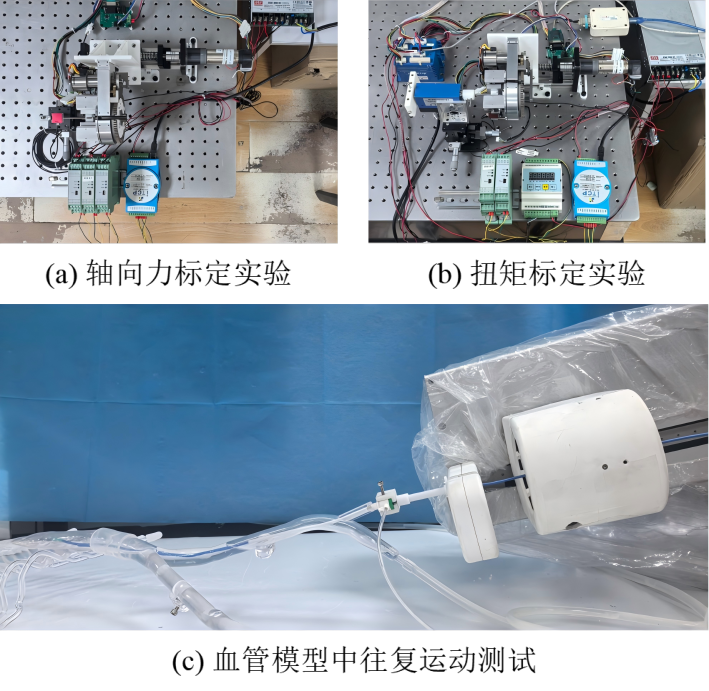
\includegraphics[width=\linewidth]{fig4.png}
\bicaption{\revised{测量参数标定与往复递送实验设置}}{\revised{Experimental configurations for measurement calibration and reciprocating delivery}}
\label{fig5}
\end{figure}

\revbegin
所有往复递送试次均在器械经导管鞘进入血管模型的同一装置中完成。推进速度设多档，指令值为 $7$～$60\,\mathrm{mm/s}$，各速度档S1与S9采用相同速度指令。各周期静止时长约为 $1.9$～$4.1\,\mathrm{s}$，插入深度随周期增加。连续递送参考的单次行程不超过 $20\,\mathrm{mm}$，覆盖统一恢复窗口 $s_{\mathrm w}$ 及相邻递送段；配对试次数、运动条件和重复次数为[待补]。
\revend

\revbegin
\subsection{载荷转移与恢复模型辨识}
\revend

\revbegin
S4和S8分别对应递送机构测力通道的卸载与重新承载。外部留出集中待恢复载荷差 $A$ 的中位数为[待补]，范围为[待补]，$A>0$ 的周期占[待补]。
\revend

\revbegin
以完整恢复模型为主，自 $s_{\mathrm r}=0.77\,\mathrm{mm}$ 起拟合（起点选择原因为[待补]），比较附加摩擦阻力项和弹性加载项的作用。外部留出集共15个文件、113个周期，其中87个周期出现局部峰值，判据为窗口内最大值相对 $\bar F$ 和末段载荷中位数的峰值超出量均至少为 $0.05\,\mathrm{N}$。不计附加摩擦阻力时，仅弹性加载模型无法给出局部峰值，相对实测恢复曲线的整窗均方根误差（RMSE）由 $0.412\,\mathrm{N}$ 升至 $0.480\,\mathrm{N}$，前 $1\,\mathrm{mm}$ 的RMSE由 $0.534\,\mathrm{N}$ 升至 $0.658\,\mathrm{N}$；完整恢复模型正确识别出其中70个局部峰值。不计弹性加载时，仅附加摩擦（$\lambda\to0$）的误差为[待补]，补偿输出在S9起始出现与待恢复载荷差相当的凹陷。校正测量及三种模型形式相对参考的S9误差分布见图\ref{fig6}(b)，辨识参数 $\lambda$、$F_{\mathrm a}$、$D_c$ 及峰位误差为[待补]。
\revend

\revbegin
恢复窗口末端载荷与切换前载荷的绝对偏差中位数约为 $0.2\,\mathrm{N}$，这部分由残差估计网络处理。
\revend

\revbegin
\begin{figure}[H]
\centering
\fbox{\parbox{0.92\linewidth}{\raggedright [待补]\par
(a) 典型周期实测S9载荷、完整恢复模型曲线及补偿后输出；\par
(b) 外部留出集上校正测量、仅附加摩擦、仅弹性加载与完整恢复模型的S9误差箱线图。}}
\bicaption{\revised{轴向载荷恢复模型辨识结果}}{\revised{Identification results of the axial load recovery model}}
\label{fig6}
\end{figure}
\revend

\revbegin
\subsection{力反馈性能评价}
\revend

\revbegin
数据按完整试次划分，连续递送参考与对应往复试次置于同一数据组，验证集用于选择超参数，外部留出集用于报告结果。测试前冻结物理参数、网络参数及标准化参数，网络采用 $M=20$ 个行程单元、$K=10$ 个历史周期和维度 $d=32$ 的单层GRU编码器与单头跨周期注意力。比较方法共六种：校正测量、保持至S8（S2～S8保持切换前载荷，S9输出校正测量）、保持至S9（S2～S9保持切换前载荷，S10输出校正测量）、恢复模型补偿、恢复模型+单周期GRU和本文方法（恢复模型+跨周期注意力残差网络）。训练与验证试次数及优化设置为[待补]，多周期轴向反馈波形及一次S9恢复反馈误差见图\ref{fig9}。
\revend

\revbegin
\begin{figure}[H]
\centering
\fbox{\parbox{0.92\linewidth}{\raggedright [待补]\par
(a) 多周期反馈波形，两机构交替承载期间的输出保持段截断显示；\par
(b) 一次S9恢复的反馈误差，对比保持至S8、保持至S9、恢复模型补偿与本文方法。}}
\bicaption{\revised{血管模型中的多周期轴向反馈重构}}{\revised{Axial force feedback reconstruction over multiple cycles in a vascular phantom}}
\label{fig9}
\end{figure}
\revend

\subsubsection{参考误差分析}

\revbegin
S9 RMSE和S9前 $1\,\mathrm{mm}$ RMSE分别为相应区间内反馈相对参考载荷的均方根误差，S2～S10误差峰峰值为该区间内反馈误差的最大值与最小值之差。S1和S10阶段各方法均输出校正测量值，其误差为[待补]。外部留出集上六种方法的轴向误差汇总于表\ref{tab1}，差异统计为[待补]。
\revend

\revbegin
\begin{table}[H]
	\centering
	\bicaption{外部留出集上的轴向力反馈误差}{Axial force feedback errors on the external held-out set}
	\label{tab1}
	\small
	\setlength{\tabcolsep}{2pt}
	\begin{tabular}{lccc}
		\toprule
		方法 & $E_{\mathrm{S9}}$/N & $E_{1\,\mathrm{mm}}$/N & $E_{\mathrm{pp}}$/N\\
		\midrule
		校正测量 & 0.7524 & 1.6052 & [待补]\\
		保持至S8 & 0.7524 & 1.6052 & [待补]\\
		保持至S9 & 0.2134 & 0.0065 & [待补]\\
		恢复模型补偿 & 0.3692 & 0.5269 & [待补]\\
		\makecell[l]{恢复模型+单周期\\GRU} & $0.3742\pm0.0155$ & $0.4926\pm0.0188$ & [待补]\\
		本文方法 & $0.3981\pm0.0320$ & $0.4949\pm0.0301$ & [待补]\\
		\bottomrule
	\end{tabular}
	\par\vspace{2pt}
		{\footnotesize 注：结果来自外部留出集（15个文件、113个周期），参考为离线构造的连续反馈目标，并非独立连续实测真值。$E_{\mathrm{S9}}$、$E_{1\,\mathrm{mm}}$ 分别为S9及其前1\,mm的RMSE；前1\,mm按当前约0.77\,mm分支起点计算。网络项为5个随机种子的均值$\pm$标准差；校正测量与保持至S8在当前S9评价窗口内输出相同。$E_{\mathrm{pp}}$ 因当前完整记录缺少可信的S2～S10精确阶段边界，暂未报告；恢复模型+单周期GRU不含跨周期注意力。}
\end{table}
\revend

\revbegin
\subsubsection{叠加阻力响应评估}
\revend

\revbegin
从外部留出集随机选取若干S9周期（周期数为[待补]），在校正测量值与参考载荷上同时叠加设定幅值的阶跃阻力和短时脉冲阻力，按各方法重新计算反馈输出，幅值、施加位置和脉冲宽度为[待补]。反馈增量取叠加前后输出之差，阶跃保留比为反馈增量平台均值与叠加幅值之比，响应延迟为反馈增量与参考增量达到叠加幅值63\%的时间差，脉冲保留比为反馈增量峰值与脉冲幅值之比。保持至S9在S9内对叠加阻力无响应，直至S10才出现；保持至S8能够保留叠加阻力，但反馈带有恢复凹陷。恢复模型补偿与本文方法的补偿量均不使用S9实时测力，叠加阻力以单位权重进入反馈，两者响应相同；阶跃与脉冲保留比及响应延迟为[待补]。低速周期在S9中叠加阶跃阻力时各方法的反馈见图\ref{fig7}。
\revend

\revbegin
\begin{figure}[H]
\centering
\fbox{\parbox{0.92\linewidth}{\raggedright [待补]\par
(a) 低速周期在S9中叠加阶跃阻力时各方法的反馈。}}
\bicaption{\revised{S9阶段叠加阻力的反馈响应}}{\revised{Feedback responses to superimposed resistance during S9}}
\label{fig7}
\end{figure}
\revend

\revbegin
\subsection{操作者实验}
\revend

\revbegin
操作者实验采用缩短后的往复夹持时序，比较未补偿反馈与本文方法；每名操作者按ABBA顺序完成两种条件各2组，且不知晓当前条件。两种条件采用相同的主端力渲染设置，力反馈比例系数 $k_f$、虚拟阻尼 $b$ 分别为[待补]和[待补]，操作者人数为[待补]。任务表现以介入总时间、通过成功率、总推进行程与路径长度之比及回撤次数评价；反馈连续性以两机构交替承载期间的输出跌落幅值、承载切换跳变幅值和S2～S10输出峰峰值评价，结果见表\ref{tab2}。各项指标以均值$\pm$标准差报告；操作者人数少于6人时不进行显著性检验，并报告各指标中本文方法占优的操作者人数，详见表注。
\revend

\revbegin
\begin{table}[H]
\centering
\bicaption{\revised{两种轴向反馈条件下的操作者实验结果}}{\revised{Operator experiment results under two axial feedback conditions}}
\label{tab2}
\small
\setlength{\tabcolsep}{2pt}
\begin{tabular}{p{0.47\linewidth}cc}
\toprule
指标 & 未补偿反馈 & 本文方法\\
\midrule
\multicolumn{3}{l}{\textbf{任务表现}}\\
介入总时间/s & [待补]$\pm$[待补] & [待补]$\pm$[待补]\\
通过成功率/% & [待补]$\pm$[待补] & [待补]$\pm$[待补]\\
总推进行程与路径长度之比 & [待补]$\pm$[待补] & [待补]$\pm$[待补]\\
回撤次数 & [待补]$\pm$[待补] & [待补]$\pm$[待补]\\
\midrule
\multicolumn{3}{l}{\textbf{反馈连续性}}\\
两机构交替承载期间输出跌落幅值/N & [待补]$\pm$[待补] & [待补]$\pm$[待补]\\
承载切换跳变幅值/N & [待补]$\pm$[待补] & [待补]$\pm$[待补]\\
S2～S10输出峰峰值/N & [待补]$\pm$[待补] & [待补]$\pm$[待补]\\
\bottomrule
\end{tabular}
\par\vspace{2pt}
{\footnotesize 注：数值为均值$\pm$标准差；操作者人数及每种条件的试次数为[待补]。反馈连续性指标根据补偿输出计算，不含主端阻尼项；通过成功率按部位次数统计。各项指标中本文方法占优的操作者人数按行序为[待补]、[待补]、[待补]、[待补]、[待补]、[待补]、[待补]。}
\end{table}
\revend

\section{讨论（Discussion）}

\revbegin
传力链弹性加载和停顿后附加摩擦阻力衰减分别对应起步段加载与局部峰值。计入附加摩擦阻力后，恢复模型能够描述局部峰值和起步段载荷变化。恢复窗口末端约 $0.2\,\mathrm{N}$ 的稳态偏差及周期间差异由残差估计网络修正；弹性加载和附加摩擦阻力作用的机理消融结果见图\ref{fig6}(b)，具体结果为[待补]。叠加阻力测试表明，补偿量与实时测力解耦，使S9阶段新增阻力不被补偿削弱。
\revend

\revbegin
按行程单元编码使不同速度下的恢复过程具有一致的表示长度，并可按行程位置对齐前序周期。表\ref{tab1}中恢复模型+单周期GRU与本文方法的比较反映跨周期注意力对残差估计的贡献，结果为[待补]。
\revend

\revbegin
本文静止时长范围较窄，附加阻力幅值与静止时长的关系、初始加载刚度与插入深度的关系均未辨识。模型结构与Dahl预滑动及速率--状态摩擦的形式一致\cite{dahl1968,ruina1983}，可通过不发生夹持状态切换的停--走试验进一步辨识。叠加阻力测试为离线叠加，实际阻力突变对接触状态的影响需结合实物加载评价。
\revend

\section{结论（Conclusions）}

\revbegin
本文建立了结合空载响应项校正、载荷转移分析、轴向载荷恢复模型和跨周期残差估计网络的力反馈重构方法。恢复模型以传力链弹性加载与停顿后附加摩擦阻力衰减描述S9的载荷变化，三个参数离线联合辨识后冻结。GRU和跨周期注意力估计恢复模型未描述的残差，结合切换期间的输出保持与补偿量平滑撤除，形成分阶段反馈。补偿量与S9实时测力解耦，离线叠加阻力可完整进入反馈；反馈重构误差及操作者实验的定量结果为[待补]。
\revend

\noindent

% -------- 参考文献表
\bibliographystyle{JQR_LaTeX_Template-0507/jqr-num}
\bibliography{JQR_LaTeX_Template-0507/references}

\begin{AuthorIntroduction}
\Intro 第一作者：隋凯丞（2000--），男，硕士研究生。研究领域：血管介入手术机器人，机器人力感知与控制。E-mail: suikaicheng24@mails.ucas.ac.cn。
\revbegin

\Intro
通信作者：胡琨元（出生年份[待补]），作者简介与E-mail为[待补]。
\revend

\Intro 通信作者：刘浩（1976--），男，博士，研究员，博士生导师。研究领域：医疗微创手术机器人，智能控制。E-mail: liuhao@sia.cn。

\end{AuthorIntroduction}

\balance
\end{document}
